\section{\CEU}
\label{sec.ceu}

\CEU is a synchronous reactive language in which programs evolve in a sequence
of discrete reactions to external events.
%
It is designed for control-intensive applications, supporting concurrent lines
of execution, known as \emph{trails}, and instantaneous broadcast communication
through events.
%
Computations within a reaction (such as expressions, assignments, and
system calls) are also instantaneous considering the synchronous
hypothesis~\cite{rp.hypothesis}.
%
%\CEU provides an \code{await} statement which is the only that actually
%``consumes'' time.
%
\CEU provides an \code{await} statement that blocks the current running trail
allowing the program to execute its other trails; when all trails are blocked,
the reaction terminates and control returns to the environment.

In \CEU, every execution path within loops must contain at least one
\code{await} statement to an external input
event~\cite{ceu.sensys13,esterel.primer}.
%
This restriction, which is statically checked by the compiler, ensures that
every reaction runs in bounded time, eventually terminating with all trails
blocked in \code{await} statements.
%
\CEU has an additional restriction, which it shares with Esterel and
synchronous languages in general~\cite{esterel.preemption}: computations that
take a non-negligible time to run (e.g., cryptography or image processing
algorithms) violate the zero-delay hypothesis, and thus cannot be directly
implemented.

Listing~\ref{lst.syntax} shows a compact reference of~\CEU:

\bgroup
\def\T<#1>{\langle\mathit{#1}\rangle}
\def\C#1#2{\hfill\rmfamily\itshape\makebox[#1\columnwidth][l]{//~#2}}
\begin{lstlisting}[
  basicstyle=\ttfamily\footnotesize,
  caption={The concrete syntax of \CEU.},
  label={lst.syntax},
]
|\C{1.}{Declarations}|
input $\T<type>$ $\T<id>$; | \C{.6}{declares an external input event} |
event $\T<type>$ $\T<id>$; | \C{.6}{declares an internal event}       |
var   $\T<type>$ $\T<id>$; | \C{.6}{declares a variable}              |

|\C{1.}{Event handling}|
$\T<id>$ = await $\T<id>$;   | \C{.6}{awaits an event and assigns the received value} |
emit $\T<id>$($\T<exp>$);    | \C{.6}{emits an event passing a value} |

|\C{1.}{Control flow}|
$\T<stmt>$ ; $\T<stmt>$                          | \C{.45}{sequence}     |
if $\T<exp>$ then $\T<stmts>$ else $\T<stmts>$ end    | \C{.45}{conditional}  |
loop do $\T<stmts>$ end                      | \C{.45}{repetition}   |
every $\T<id>$ in $\T<id>$ do $\T<stmts>$ end         | \C{.45}{event iteration}   |
finalize [$\T<stmts>$] with $\T<stmts>$ end       | \C{.45}{finalization} |

|\C{1.}{Logical parallelism}|
par/or  do $\T<stmts>$ with $\T<stmts>$ end | \C{.45}{aborts when any side ends}      |
par/and do $\T<stmts>$ with $\T<stmts>$ end | \C{.45}{terminates when all sides ends} |

|\C{1.}{Assignment \& Integration with C}|
$\T<id>$ = $\T<exp>$; | \C{.6}{assigns a value to a variable}              |
_$\T<id>$($\T<exps>$) | \C{.6}{calls a C function (id starts with `\_'\,)} |
\end{lstlisting}
\egroup

Listing~\ref{lst.ceu} shows a complete example in \CEU that toggles a LED
whenever a radio packet is received, terminating with a button press always
with the LED off.
%
The implementation first declares the \code{BUTTON} and \code{RADIO\_RECV} as
input events (ln.~1--2).
Then, it uses a \code{par/or} composition to run two activities in parallel:
a single-statement trail that waits for a button press before terminating
(ln.~4), and an endless loop that toggles the LED on and off on radio receives
(ln.~9--14).
The \code{finalize} clause (ln.~6--8) ensures that, no matter how its enclosing
trail terminates, the LED will be unconditionally turned off (ln.~7).

The \code{par/or} composition, which stands for a \emph{parallel-or}, provides
an orthogonal abortion mechanism~\cite{esterel.preemption} in which its
composed trails do not know when and how they are aborted (i.e., abortion is
external to them).
%
%This is possible to do safely in synchronous languages due to the accurate
%control of concurrent activities, i.e., in between every reaction, the whole
%system is idle and consistent~\cite{esterel.preemption}.
%
The finalization mechanism extends orthogonal abortion to also work with
activities that use stateful resources from the environment (such as files and
network handlers), as we discuss in Section~\ref{sec.ceu.fin}.
%

\begin{lstlisting}[
  numbers=left,
  basicstyle=\ttfamily\footnotesize,
  float=h,
  caption={A program in \CEU that toggles a LED on every radio receive,
           terminating on a button press always with the LED off.},
  label={lst.ceu},
]
input void BUTTON;
input void RADIO_RECV;
par/or do
    await BUTTON;
with
    finalize with
        _led(0);
    end
    loop do
        _led(1);
        await RADIO_RECV;
        _led(0);
        await RADIO_RECV;
    end
end
\end{lstlisting}

In \CEU, any identifier prefixed with an underscore (e.g., \code{\_led}) is
passed unchanged to the underlying~C compiler.
%
Therefore, access to~C is straightforward and syntactically traceable.
%
To ensure that programs operate under the synchronous hypothesis, the compiler
environment should only provide access to~C operations that can be assumed to
be instantaneous, such as non-blocking~I/O and simple data structure accessors.

\subsection{External and Internal Events}
\label{sec.ceu.evts}

\CEU defines time as a discrete sequence of reactions to unique external
input events received from the environment.
%
Each input event delimits a new logical unit of time that triggers an
associated reaction.
%
The life-cycle of a program in \CEU can be summarized as
follows~\cite{ceu.sensys13}:
%
\begin{enumerate}[i]
\item The program initiates a ``boot reaction'' in a single trail (parallel
      constructs may create new trails).
\item Active trails execute until they await or terminate, one after
      another.  This step is called a \emph{reaction chain}, and always runs in
      bounded time.
\item When all trails are blocked, the program goes idle and the environment
      takes control.
\item On the occurrence of a new external input event, the environment
      awakes \emph{all} trails awaiting that event, and the program goes back to
      step~(ii).
\end{enumerate}

A program must react to an event completely before handling the next one.
%
By the synchronous hypothesis, the time the program spends in step~(ii) is
conceptually zero (in practice, negligible).
%
Hence, from the point of view of the environment, the program is always
idle on step~(iii).
%
In practice, if a new external input event occurs while a reaction executes,
the event is saved on a queue, which effectively schedules it to be processed
in a subsequent reaction.

\subsubsection*{External events and discrete time}

\begin{figure}[b]
\centering
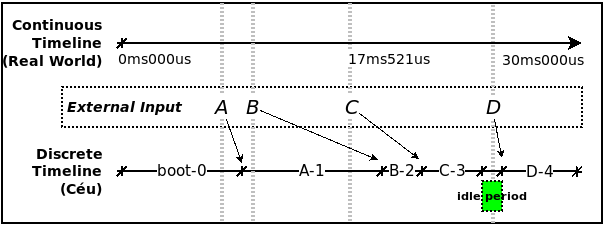
\includegraphics[width=\columnwidth]{tick_min}
\caption{The discrete notion of time in \CEU.}
\label{fig.ticks}
\end{figure}

The sequential processing of external input events induces a discrete notion of
time in \CEU, as illustrated in Figure~\ref{fig.ticks}.
%
The continuous timeline shows an absolute reference clock with ``physical
timestamps'' for the event occurrences (e.g., event~\code{C} occurs at
$17ms521us$).
%
The discrete timeline shows how the same occurring events fit in the logical
notion of time of \CEU.
%
The boot reaction \code{boot-0} happens before any input, at program startup.
%
Event~\code{A} ``physically'' occurs during \code{boot-0} but, because time
is discrete, its corresponding reaction only executes afterwards, at logical
instant~\code{A-1}.
%
Similarly, event~\code{B} occurs during~\code{A-1} and its reaction is
postponed to execute at~\code{B-2}.
%
Event~\code{C} also occurs during~\code{A-1} but its reaction must also wait
for~\code{B-2} to execute and so it is postponed to execute at~\code{C-3}.
%
Finally, event~\code{D} occurs during an idle period and can start immediately
at \code{D-4}.
%
%Finally, two instances of event~\code{E} occur during~\code{D-4}; they are
%handled in the subsequent reactions~\code{E-5} and~\code{E-6}.

Unique input events imply mutually exclusive reactions, which execute
atomically and never overlap.
%
Automatic mutual exclusion is a prerequisite for deterministic reactions as
we discuss in Section~\ref{sec.sem}.
%
%8<- - - - - - - - - - - - - - - - - - - - - - - - - - - - - - - - - - - - -
% \gl{A não ser que seja desenvolvido (e.g., explicado e comparado com
%   Esterel) eu acho que o parágrafo anterior é dispensável.}
% \fs{Tirei o "simplifies resoning about concurrency".
%     O resto do parágrafo é absoluto e tenta dar a intuição das condições para
%     ter determinismo.}
%- - - - - - - - - - - - - - - - - - - - - - - - - - - - - - - - - - - - ->8

In practice, the synchronous hypothesis for \CEU holds if reactions execute
faster than the rate of incoming input events.
%
Otherwise, the program would continuously accumulate delays between physical
occurrences and actual reactions for the input events.
%
Considering the context of soft real-time systems,
%targeted by \CEU (e.g., sensor networks, multimedia systems, interactive games, etc.)
postponed reactions might be tolerated as long as they are infrequent and the
application does not take too long to catch up with real time.
%
Note that the synchronous semantics is also the norm in typical event-driven
systems, such as event dispatching in UI toolkits, game loops in game engines,
and clock ticks in embedded systems.

\subsubsection*{Internal events as subroutines}

In \CEU, queue-based processing of events applies only to external input
events, i.e., events submitted to the program by the environment.
%
Internal events, which are events generated internally by the program via
\code{emit} statements, are processed in a stack-based manner.
%
Internal events provide a fine-grained execution control, and, because of their
stack-based processing, can be used to implement a limited form of subroutines,
as illustrated in Listing~\ref{lst.sub}:

\begin{lstlisting}[
  numbers=left,
  basicstyle=\ttfamily\footnotesize,
  float=h,
  caption={A \CEU program with a ``subroutine''.},
  label={lst.sub},
]
event int* inc;         // declares subroutine "inc"
par/or do
    var int* p;
    every p in inc do   // implements "inc" through an event iterator
        *p = *p + 1;
    end
with
    var int v = 1;
    emit inc(&v);       // calls "inc"
    emit inc(&v);       // calls "inc"
    _assert(v==3);      // asserts result after the two returns
end
\end{lstlisting}
%\vskip-\baselineskip

In the example, the ``subroutine'' \code{inc} is defined as an event iterator
(ln.~4--6) that continuously awaits its identifying event (ln.~4), and
increments the value passed by reference (ln.~5).
%
A trail in parallel (ln.~8--11) invokes the subroutine through two consecutive
\code{emit} statements (ln.~9--10).
%
Given the stack-based execution for internal events, as the first emit
executes, the calling trail pauses (ln.~9), the subroutine awakes (ln.~4), runs
its body (yielding \code{v=2}), iterates, and awaits the next ``call'' (ln.~4,
again).
%
Only after this sequence does the calling trail resumes (ln.~9), makes a new
invocation (ln.~10), and passes the assertion test (ln.~11).

%- multiple executions
%- footnote to distinguish from TECS

\CEU also supports nested \code{emit} invocations, e.g., the body of the
subroutine \code{inc} (ln.~5) could \code{emit} an event targeting another
subroutine, creating a new level in the stack.
%
We can think of the stack as a record of the nested, fine-grained internal
reactions that happen inside the same outer reaction to a single external
event.

This form of subroutines has a significant limitation that it cannot express
recursion, since an \code{emit} to itself is always ignored as a running trail
cannot be waiting on itself.
%
That being said, it is this very limitation that brings important safety
properties to subroutines.
%
First, they are guaranteed to react in bounded time.
%
Second, memory for locals is also bounded, not requiring data stacks.

At first sight, event iteration such as in ``\code{every e do <...> end}'' seems
to be equivalent to ``\code{loop do await e; <...> end}''.
However, the \code{loop} variation would not compile because it does not
contain a path to an external input \code{await} (since \code{e} is an internal
event).
%
However, event iterators enforce other syntactic restrictions and cannot
contain \code{await} or \code{break} statements.
The absence of \code{break} guarantees that an iterator never terminates from
itself, essentially behaving as a safe blocking point in the program.
%
For this reason, the restriction that execution paths within loops must
contain at least one external \code{await} is extended to alternatively contain
an \code{every} statement.

\subsection{Shared-Memory Concurrency}
\label{sec.ceu.shared}

Embedded applications make extensive use of global memory and shared resources,
such as through memory-mapped registers and system calls to device drivers.
Hence, an important goal of \CEU is to ensure a reliable behavior for programs
with concurrent lines of execution sharing memory and interacting with the
environment.

\begin{figure}[h]
\begin{minipage}[h]{0.45\linewidth}
\begin{lstlisting}[numbers=right]
input void A;
input void B;
var int x = 1;
par/and do
    await A;
    x = x + 1;
with
    await B;
    x = x * 2;
end
\end{lstlisting}
\centering\small{\ax Accesses to \code{x} are never concurrent.}
\end{minipage}
%
\begin{minipage}[h]{0.53\linewidth}
%\begin{lstlisting}
\begin{lstlisting}[xleftmargin=2em]
input void A;
// (empty line)
var int y = 1;
par/and do
    await A;
    y = y + 1;
with
    await A;
    y = y * 2;
end

\end{lstlisting}
\centering\small{\bx Accesses to \code{y} are concurrent but still deterministic.}
\end{minipage}
%\rule{8.4cm}{0.37pt}
\caption{ Shared-memory concurrency in \CEU:
example \ax is safe because the trails access \code{x} atomically in different
reactions;
example \bx is unsafe because both trails access \code{y} in the same reaction.
\label{lst.shared}
}
\end{figure}

In \CEU, when multiple trails are active during the same reaction, they are
scheduled in lexical order, i.e., in the order they appear in the program
source code.
%
For instance, consider the two examples in Figure~\ref{lst.shared}, both
defining shared variables (ln. 3), and assigning to them in parallel trails
(ln. 6, 9).

In the example \ax, the two assignments to \code{x} can only execute in
reactions to different events \code{A} and \code{B} (ln. 5,8), which cannot
occur simultaneously by definition.
Hence, for the sequence of events \code{A->B}, \code{x} becomes \code{4}
(\code{(1+1)*2}), while for \code{B->A}, \code{x} becomes \code{3}
(\code{(1*2)+1}).

In the example \bx, the two assignments to \code{y} are simultaneous because
they execute in reaction to the same event \code{A}.
Since \CEU employs lexical order for intra-reaction statements, the execution
is still deterministic, and \code{y} always becomes \code{4} (\code{(1+1)*2}).
%
However, note that an apparently innocuous change in the order of trails
modifies the behavior of the program.
%
To mitigate this threat, \CEU performs concurrency checks at compile time to
detect conflicting accesses to shared variables:
if a variable is written in a trail segment, then a concurrent trail segment
cannot read or write to that variable~\cite{ceu.sensys13}.
%
Nonetheless, the static checks are optional and are not a prerequisite for the
deterministic semantics of the language.

\subsection{Abortion and Finalization}
\label{sec.ceu.fin}

\begin{figure}
\begin{minipage}[t]{0.45\linewidth}
\begin{lstlisting}[numbers=right]
par/or do
   var _msg_t msg;
   <...> // prepare msg
   finalize
      _send(&msg);
   with
      _cancel(&msg);
   end
   await SEND_ACK;
with
   <...>
end
//
\end{lstlisting}
\centering\small{\ax Local resource finalization}
\end{minipage}
%
\begin{minipage}[t]{0.53\linewidth}
\begin{lstlisting}[xleftmargin=2em]
par/or do
   var _FILE* f;
   finalize
      f = _fopen(...);
   with
      _fclose(f);
   end
   _fwrite(..., f);
   await A;
   _fwrite(..., f);
with
   <...>
end
\end{lstlisting}
\centering\small{\bx External resource finalization}
\end{minipage}
%\rule{8.4cm}{0.37pt}
\caption{
\CEU enforces the use of finalization to prevent \emph{dangling pointers} for
local resources and \emph{memory leaks} for external resources.
\label{lst.fin.ceu}
}
\end{figure}

The \code{par/or} of \CEU is an orthogonal abortion mechanism because the two
sides in the composition need not be tweaked with synchronization primitives or
state variables in order to affect each other.
%
In addition, abortion is \emph{immediate} in the sense that it executes
atomically in the current micro reaction.
%
Immediate orthogonal abortion is a distinctive feature of synchronous languages
and cannot be expressed effectively in traditional (asynchronous)
multi-threaded languages~\cite{esterel.preemption,sync_async.threadsstop}.

However, aborting lines of execution that deal with external resources may lead
to inconsistencies.
%
For this reason, \CEU provides a \code{finalize} construct to unconditionally
execute a series of statements even if the enclosing block is externally
aborted.

\CEU also enforces the use of \code{finalize} for system calls that deal with
pointers representing resources, as illustrated in the two examples of
Figure~\ref{lst.fin.ceu}:
%
\begin{itemize}
    \item If \CEU \textbf{passes} a pointer to a system call (ln. \ax:5), the
          pointer represents a \textbf{local} resource (ln. \ax:2) that
          requires finalization (ln. \ax:7).
    \item If \CEU \textbf{receives} a pointer from a system call return
          (ln.  \bx:4), the pointer represents an \textbf{external} resource
          (ln. \bx:2) that requires finalization (ln. \bx:6).
\end{itemize}
%
\CEU tracks the interaction of system calls with pointers and requires
finalization clauses to accompany them.
%
In the example in Figure~\ref{lst.fin.ceu}.a, the local variable \code{msg}
(ln. 2) is an internal resource passed as a pointer to \code{\_send} (ln. 5),
which is an asynchronous call that transmits the buffer in the background.
If the block aborts (ln. 11) before receiving an acknowledge from the
environment (ln. 9), the local \code{msg} goes out of scope and the external
transmission now holds a \emph{dangling pointer}.
The finalization ensures that the transmission also aborts (ln. 7).
%
In the example in Figure~\ref{lst.fin.ceu}.b, the call to \code{\_fopen} (ln.
4) returns an external file resource as a pointer.
If the block aborts (ln. 12) during the \code{await A} (ln. 9), the file
remains open as a \emph{memory leak}.
The finalization ensures that the file closes properly (ln. 6).
%
In both cases, the code does not compile without the \code{finalize}
construct.%
\footnote{
The compiler only forces the programmer to write the finalization clause, but
cannot check if it actually handles the resource properly.
}

The finalization mechanism of \CEU is fundamental to preserve the orthogonality
of the \code{par/or} construct since the clean up code is encapsulated in the
aborted trail itself.
